\documentclass{standalone}
\usepackage{tikz}
\usetikzlibrary{patterns, positioning}

\begin{document}
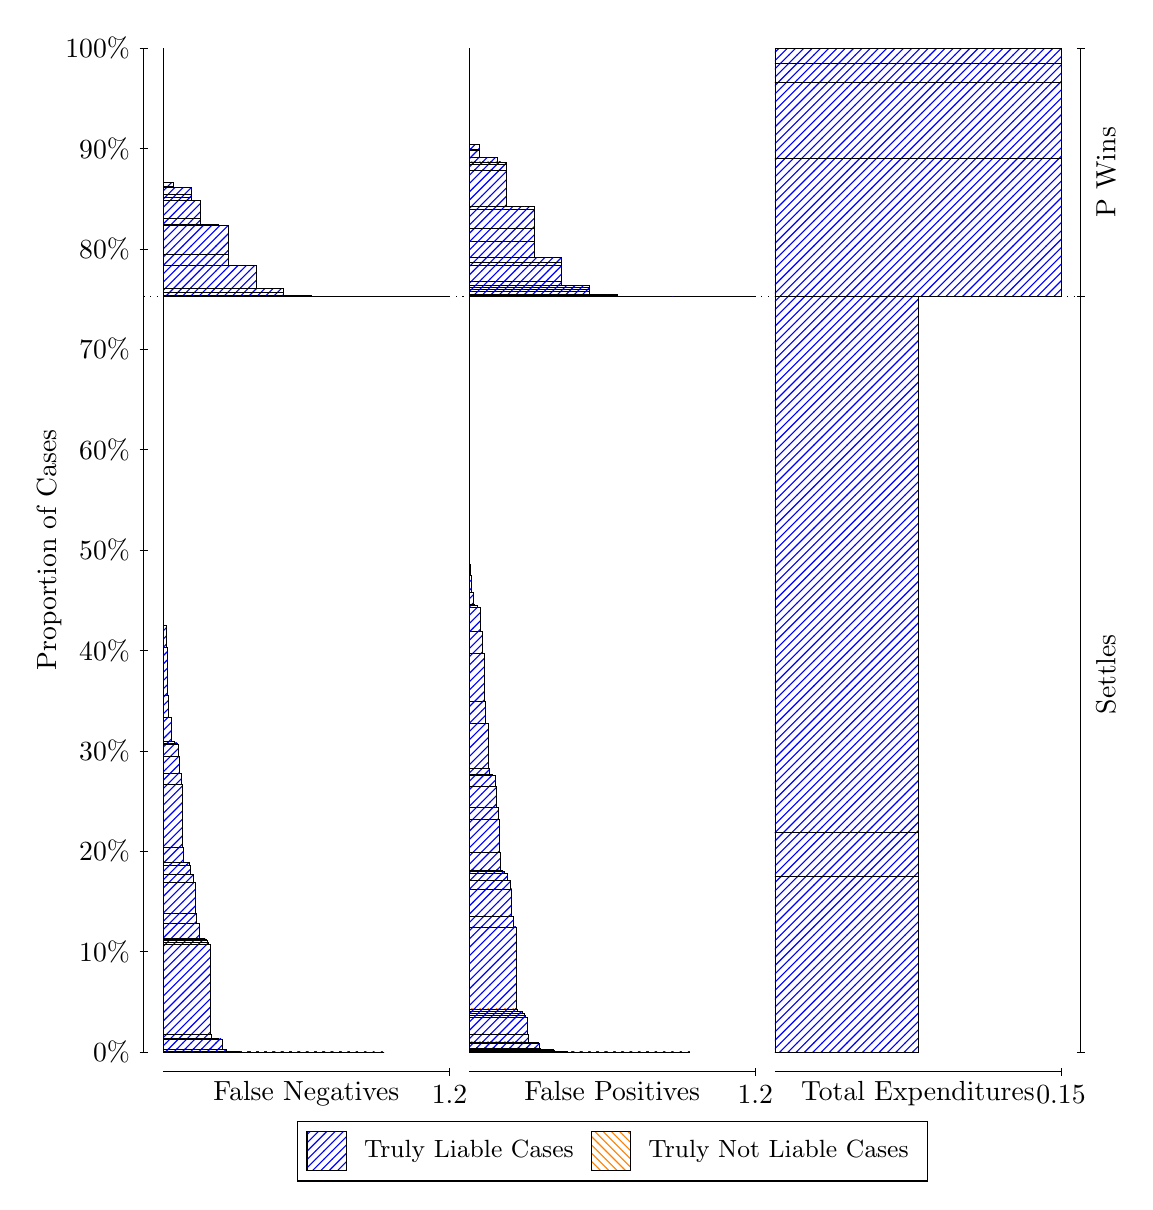
\begin{tikzpicture}
\draw[black, very thin] (1.5,1.75) -- (1.5,14.5);
\node[rotate=90, anchor=center] at (0.3, 8.125) {Proportion of Cases};
\draw[black, very thin] (1.45,1.75) -- (1.55,1.75);
\node[anchor=east] at (1.45, 1.75) {0\%};
\draw[black, very thin] (1.45,3.025) -- (1.55,3.025);
\node[anchor=east] at (1.45, 3.025) {10\%};
\draw[black, very thin] (1.45,4.3) -- (1.55,4.3);
\node[anchor=east] at (1.45, 4.3) {20\%};
\draw[black, very thin] (1.45,5.575) -- (1.55,5.575);
\node[anchor=east] at (1.45, 5.575) {30\%};
\draw[black, very thin] (1.45,6.85) -- (1.55,6.85);
\node[anchor=east] at (1.45, 6.85) {40\%};
\draw[black, very thin] (1.45,8.125) -- (1.55,8.125);
\node[anchor=east] at (1.45, 8.125) {50\%};
\draw[black, very thin] (1.45,9.4) -- (1.55,9.4);
\node[anchor=east] at (1.45, 9.4) {60\%};
\draw[black, very thin] (1.45,10.675) -- (1.55,10.675);
\node[anchor=east] at (1.45, 10.675) {70\%};
\draw[black, very thin] (1.45,11.95) -- (1.55,11.95);
\node[anchor=east] at (1.45, 11.95) {80\%};
\draw[black, very thin] (1.45,13.225) -- (1.55,13.225);
\node[anchor=east] at (1.45, 13.225) {90\%};
\draw[black, very thin] (1.45,14.5) -- (1.55,14.5);
\node[anchor=east] at (1.45, 14.5) {100\%};

\draw[black, very thin] (13.4,1.75) -- (13.4,14.5);
\draw[black, very thin] (13.35,1.75) -- (13.45,1.75);
\node[anchor=west] at (13.35, 1.75) {};
\draw[black, very thin] (13.35,11.343) -- (13.45,11.343);
\node[anchor=west] at (13.35, 11.343) {};
\draw[black, very thin] (13.35,14.5) -- (13.45,14.5);
\node[anchor=west] at (13.35, 14.5) {};

\draw[black, very thin, pattern color=blue, pattern=north east lines] (1.75,1.75) rectangle (4.554,1.75);
\draw[black, very thin, pattern color=blue, pattern=north east lines] (1.75,1.75) rectangle (4.396,1.75);
\draw[black, very thin, pattern color=blue, pattern=north east lines] (1.75,1.75) rectangle (4.238,1.75);
\draw[black, very thin, pattern color=blue, pattern=north east lines] (1.75,1.75) rectangle (4.2029,1.75);
\draw[black, very thin, pattern color=blue, pattern=north east lines] (1.75,1.75) rectangle (4.0801,1.75);
\draw[black, very thin, pattern color=blue, pattern=north east lines] (1.75,1.75) rectangle (4.045,1.75);
\draw[black, very thin, pattern color=blue, pattern=north east lines] (1.75,1.75) rectangle (3.9221,1.75);
\draw[black, very thin, pattern color=blue, pattern=north east lines] (1.75,1.75) rectangle (3.887,1.75);
\draw[black, very thin, pattern color=blue, pattern=north east lines] (1.75,1.75) rectangle (3.8519,1.75);
\draw[black, very thin, pattern color=blue, pattern=north east lines] (1.75,1.75) rectangle (3.7641,1.75);
\draw[black, very thin, pattern color=blue, pattern=north east lines] (1.75,1.75) rectangle (3.729,1.75);
\draw[black, very thin, pattern color=blue, pattern=north east lines] (1.75,1.75) rectangle (3.6939,1.75);
\draw[black, very thin, pattern color=blue, pattern=north east lines] (1.75,1.75) rectangle (3.6062,1.75);
\draw[black, very thin, pattern color=blue, pattern=north east lines] (1.75,1.75) rectangle (3.5711,1.75);
\draw[black, very thin, pattern color=blue, pattern=north east lines] (1.75,1.75) rectangle (3.536,1.75);
\draw[black, very thin, pattern color=blue, pattern=north east lines] (1.75,1.75) rectangle (3.5008,1.75);
\draw[black, very thin, pattern color=blue, pattern=north east lines] (1.75,1.75) rectangle (3.4482,1.75);
\draw[black, very thin, pattern color=blue, pattern=north east lines] (1.75,1.75) rectangle (3.4131,1.75);
\draw[black, very thin, pattern color=blue, pattern=north east lines] (1.75,1.75) rectangle (3.378,1.75);
\draw[black, very thin, pattern color=blue, pattern=north east lines] (1.75,1.75) rectangle (3.3429,1.75);
\draw[black, very thin, pattern color=blue, pattern=north east lines] (1.75,1.75) rectangle (3.2902,1.75);
\draw[black, very thin, pattern color=blue, pattern=north east lines] (1.75,1.75) rectangle (3.2551,1.75);
\draw[black, very thin, pattern color=blue, pattern=north east lines] (1.75,1.75) rectangle (3.22,1.75);
\draw[black, very thin, pattern color=blue, pattern=north east lines] (1.75,1.75) rectangle (3.1849,1.75);
\draw[black, very thin, pattern color=blue, pattern=north east lines] (1.75,1.75) rectangle (3.1498,1.75);
\draw[black, very thin, pattern color=blue, pattern=north east lines] (1.75,1.75) rectangle (3.1322,1.75);
\draw[black, very thin, pattern color=blue, pattern=north east lines] (1.75,1.75) rectangle (3.0971,1.75);
\draw[black, very thin, pattern color=blue, pattern=north east lines] (1.75,1.75) rectangle (3.062,1.75);
\draw[black, very thin, pattern color=blue, pattern=north east lines] (1.75,1.75) rectangle (3.0269,1.75);
\draw[black, very thin, pattern color=blue, pattern=north east lines] (1.75,1.75) rectangle (2.9918,1.75);
\draw[black, very thin, pattern color=blue, pattern=north east lines] (1.75,1.75) rectangle (2.9743,1.75);
\draw[black, very thin, pattern color=blue, pattern=north east lines] (1.75,1.75) rectangle (2.9392,1.75);
\draw[black, very thin, pattern color=blue, pattern=north east lines] (1.75,1.75) rectangle (2.9041,1.7505);
\draw[black, very thin, pattern color=blue, pattern=north east lines] (1.75,1.7505) rectangle (2.869,1.7507);
\draw[black, very thin, pattern color=blue, pattern=north east lines] (1.75,1.7507) rectangle (2.8339,1.7507);
\draw[black, very thin, pattern color=blue, pattern=north east lines] (1.75,1.7507) rectangle (2.7988,1.7508);
\draw[black, very thin, pattern color=blue, pattern=north east lines] (1.75,1.7508) rectangle (2.7812,1.7508);
\draw[black, very thin, pattern color=blue, pattern=north east lines] (1.75,1.7508) rectangle (2.7461,1.7508);
\draw[black, very thin, pattern color=blue, pattern=north east lines] (1.75,1.7508) rectangle (2.711,1.7531);
\draw[black, very thin, pattern color=blue, pattern=north east lines] (1.75,1.7531) rectangle (2.6759,1.7538);
\draw[black, very thin, pattern color=blue, pattern=north east lines] (1.75,1.7538) rectangle (2.6583,1.7548);
\draw[black, very thin, pattern color=blue, pattern=north east lines] (1.75,1.7548) rectangle (2.6408,1.7553);
\draw[black, very thin, pattern color=blue, pattern=north east lines] (1.75,1.7553) rectangle (2.6232,1.7556);
\draw[black, very thin, pattern color=blue, pattern=north east lines] (1.75,1.7556) rectangle (2.5881,1.7557);
\draw[black, very thin, pattern color=blue, pattern=north east lines] (1.75,1.7557) rectangle (2.553,1.7791);
\draw[black, very thin, pattern color=blue, pattern=north east lines] (1.75,1.7791) rectangle (2.5179,1.7885);
\draw[black, very thin, pattern color=blue, pattern=north east lines] (1.75,1.7885) rectangle (2.5004,1.9106);
\draw[black, very thin, pattern color=blue, pattern=north east lines] (1.75,1.9106) rectangle (2.4828,1.9172);
\draw[black, very thin, pattern color=blue, pattern=north east lines] (1.75,1.9172) rectangle (2.4477,1.9228);
\draw[black, very thin, pattern color=blue, pattern=north east lines] (1.75,1.9228) rectangle (2.4302,1.9249);
\draw[black, very thin, pattern color=blue, pattern=north east lines] (1.75,1.9249) rectangle (2.395,1.925);
\draw[black, very thin, pattern color=blue, pattern=north east lines] (1.75,1.925) rectangle (2.3599,1.9733);
\draw[black, very thin, pattern color=blue, pattern=north east lines] (1.75,1.9733) rectangle (2.3424,3.1148);
\draw[black, very thin, pattern color=blue, pattern=north east lines] (1.75,3.1148) rectangle (2.3248,3.1384);
\draw[black, very thin, pattern color=blue, pattern=north east lines] (1.75,3.1384) rectangle (2.3073,3.1657);
\draw[black, very thin, pattern color=blue, pattern=north east lines] (1.75,3.1657) rectangle (2.2897,3.1863);
\draw[black, very thin, pattern color=blue, pattern=north east lines] (1.75,3.1863) rectangle (2.2722,3.1915);
\draw[black, very thin, pattern color=blue, pattern=north east lines] (1.75,3.1915) rectangle (2.2371,3.1946);
\draw[black, very thin, pattern color=blue, pattern=north east lines] (1.75,3.1946) rectangle (2.202,3.3871);
\draw[black, very thin, pattern color=blue, pattern=north east lines] (1.75,3.3871) rectangle (2.1669,3.5099);
\draw[black, very thin, pattern color=blue, pattern=north east lines] (1.75,3.5099) rectangle (2.1493,3.901);
\draw[black, very thin, pattern color=blue, pattern=north east lines] (1.75,3.901) rectangle (2.1318,4.0081);
\draw[black, very thin, pattern color=blue, pattern=north east lines] (1.75,4.0081) rectangle (2.0967,4.1261);
\draw[black, very thin, pattern color=blue, pattern=north east lines] (1.75,4.1261) rectangle (2.0791,4.158);
\draw[black, very thin, pattern color=blue, pattern=north east lines] (1.75,4.158) rectangle (2.044,4.1599);
\draw[black, very thin, pattern color=blue, pattern=north east lines] (1.75,4.1599) rectangle (2.0089,4.3524);
\draw[black, very thin, pattern color=blue, pattern=north east lines] (1.75,4.3524) rectangle (1.9913,5.1448);
\draw[black, very thin, pattern color=blue, pattern=north east lines] (1.75,5.1448) rectangle (1.9738,5.2885);
\draw[black, very thin, pattern color=blue, pattern=north east lines] (1.75,5.2885) rectangle (1.9562,5.5024);
\draw[black, very thin, pattern color=blue, pattern=north east lines] (1.75,5.5024) rectangle (1.9387,5.6518);
\draw[black, very thin, pattern color=blue, pattern=north east lines] (1.75,5.6518) rectangle (1.9211,5.6756);
\draw[black, very thin, pattern color=blue, pattern=north east lines] (1.75,5.6756) rectangle (1.886,5.6948);
\draw[black, very thin, pattern color=blue, pattern=north east lines] (1.75,5.6948) rectangle (1.8509,6.0003);
\draw[black, very thin, pattern color=blue, pattern=north east lines] (1.75,6.0003) rectangle (1.8158,6.2806);
\draw[black, very thin, pattern color=blue, pattern=north east lines] (1.75,6.2806) rectangle (1.7983,6.8868);
\draw[black, very thin, pattern color=blue, pattern=north east lines] (1.75,6.8868) rectangle (1.7807,7.1704);
\draw[black, very thin, pattern color=orange, pattern=north west lines] (1.75,7.1704) rectangle (1.75,7.1704);
\draw[black, very thin, pattern color=blue, pattern=north east lines] (1.75,7.1704) rectangle (1.75,11.343);
\draw[black, very thin, pattern color=blue, pattern=north east lines] (1.75,11.343) rectangle (5.3833,11.343);
\draw[black, very thin, pattern color=blue, pattern=north east lines] (1.75,11.343) rectangle (5.0323,11.343);
\draw[black, very thin, pattern color=blue, pattern=north east lines] (1.75,11.343) rectangle (5.0323,11.343);
\draw[black, very thin, pattern color=blue, pattern=north east lines] (1.75,11.343) rectangle (4.6812,11.343);
\draw[black, very thin, pattern color=blue, pattern=north east lines] (1.75,11.343) rectangle (4.6812,11.343);
\draw[black, very thin, pattern color=blue, pattern=north east lines] (1.75,11.343) rectangle (4.3302,11.343);
\draw[black, very thin, pattern color=blue, pattern=north east lines] (1.75,11.343) rectangle (4.2073,11.343);
\draw[black, very thin, pattern color=blue, pattern=north east lines] (1.75,11.343) rectangle (3.9791,11.344);
\draw[black, very thin, pattern color=blue, pattern=north east lines] (1.75,11.344) rectangle (3.9791,11.345);
\draw[black, very thin, pattern color=blue, pattern=north east lines] (1.75,11.345) rectangle (3.8563,11.345);
\draw[black, very thin, pattern color=blue, pattern=north east lines] (1.75,11.345) rectangle (3.8563,11.345);
\draw[black, very thin, pattern color=blue, pattern=north east lines] (1.75,11.345) rectangle (3.6281,11.361);
\draw[black, very thin, pattern color=blue, pattern=north east lines] (1.75,11.361) rectangle (3.5052,11.361);
\draw[black, very thin, pattern color=blue, pattern=north east lines] (1.75,11.361) rectangle (3.2771,11.392);
\draw[black, very thin, pattern color=blue, pattern=north east lines] (1.75,11.392) rectangle (3.2771,11.449);
\draw[black, very thin, pattern color=blue, pattern=north east lines] (1.75,11.449) rectangle (3.1542,11.449);
\draw[black, very thin, pattern color=blue, pattern=north east lines] (1.75,11.449) rectangle (3.1542,11.449);
\draw[black, very thin, pattern color=blue, pattern=north east lines] (1.75,11.449) rectangle (2.926,11.743);
\draw[black, very thin, pattern color=blue, pattern=north east lines] (1.75,11.743) rectangle (2.8031,11.744);
\draw[black, very thin, pattern color=blue, pattern=north east lines] (1.75,11.744) rectangle (2.8031,11.744);
\draw[black, very thin, pattern color=blue, pattern=north east lines] (1.75,11.744) rectangle (2.8031,11.744);
\draw[black, very thin, pattern color=blue, pattern=north east lines] (1.75,11.744) rectangle (2.575,11.881);
\draw[black, very thin, pattern color=blue, pattern=north east lines] (1.75,11.881) rectangle (2.575,12.243);
\draw[black, very thin, pattern color=blue, pattern=north east lines] (1.75,12.243) rectangle (2.4521,12.244);
\draw[black, very thin, pattern color=blue, pattern=north east lines] (1.75,12.244) rectangle (2.4521,12.259);
\draw[black, very thin, pattern color=blue, pattern=north east lines] (1.75,12.259) rectangle (2.2239,12.332);
\draw[black, very thin, pattern color=blue, pattern=north east lines] (1.75,12.332) rectangle (2.2239,12.568);
\draw[black, very thin, pattern color=blue, pattern=north east lines] (1.75,12.568) rectangle (2.101,12.607);
\draw[black, very thin, pattern color=blue, pattern=north east lines] (1.75,12.607) rectangle (2.101,12.641);
\draw[black, very thin, pattern color=blue, pattern=north east lines] (1.75,12.641) rectangle (2.101,12.735);
\draw[black, very thin, pattern color=blue, pattern=north east lines] (1.75,12.735) rectangle (1.8729,12.735);
\draw[black, very thin, pattern color=blue, pattern=north east lines] (1.75,12.735) rectangle (1.8729,12.741);
\draw[black, very thin, pattern color=blue, pattern=north east lines] (1.75,12.741) rectangle (1.8729,12.789);
\draw[black, very thin, pattern color=blue, pattern=north east lines] (1.75,12.789) rectangle (1.8729,12.789);
\draw[black, very thin, pattern color=orange, pattern=north west lines] (1.75,12.789) rectangle (1.75,12.789);
\draw[black, very thin, pattern color=blue, pattern=north east lines] (1.75,12.789) rectangle (1.75,14.5);
\draw[black, very thin, pattern color=orange, pattern=north west lines] (5.6333,1.75) rectangle (8.4373,1.75);
\draw[black, very thin, pattern color=blue, pattern=north east lines] (5.6333,1.75) rectangle (8.4373,1.75);
\draw[black, very thin, pattern color=orange, pattern=north west lines] (5.6333,1.75) rectangle (8.2793,1.75);
\draw[black, very thin, pattern color=blue, pattern=north east lines] (5.6333,1.75) rectangle (8.2793,1.75);
\draw[black, very thin, pattern color=orange, pattern=north west lines] (5.6333,1.75) rectangle (8.1214,1.75);
\draw[black, very thin, pattern color=blue, pattern=north east lines] (5.6333,1.75) rectangle (8.1214,1.75);
\draw[black, very thin, pattern color=blue, pattern=north east lines] (5.6333,1.75) rectangle (8.0863,1.75);
\draw[black, very thin, pattern color=blue, pattern=north east lines] (5.6333,1.75) rectangle (7.9283,1.75);
\draw[black, very thin, pattern color=orange, pattern=north west lines] (5.6333,1.75) rectangle (7.8054,1.75);
\draw[black, very thin, pattern color=blue, pattern=north east lines] (5.6333,1.75) rectangle (7.8054,1.75);
\draw[black, very thin, pattern color=blue, pattern=north east lines] (5.6333,1.75) rectangle (7.7703,1.75);
\draw[black, very thin, pattern color=blue, pattern=north east lines] (5.6333,1.75) rectangle (7.7352,1.75);
\draw[black, very thin, pattern color=orange, pattern=north west lines] (5.6333,1.75) rectangle (7.6475,1.75);
\draw[black, very thin, pattern color=blue, pattern=north east lines] (5.6333,1.75) rectangle (7.6475,1.75);
\draw[black, very thin, pattern color=blue, pattern=north east lines] (5.6333,1.75) rectangle (7.5773,1.75);
\draw[black, very thin, pattern color=orange, pattern=north west lines] (5.6333,1.75) rectangle (7.4895,1.75);
\draw[black, very thin, pattern color=blue, pattern=north east lines] (5.6333,1.75) rectangle (7.4895,1.75);
\draw[black, very thin, pattern color=blue, pattern=north east lines] (5.6333,1.75) rectangle (7.4544,1.75);
\draw[black, very thin, pattern color=blue, pattern=north east lines] (5.6333,1.75) rectangle (7.4193,1.75);
\draw[black, very thin, pattern color=blue, pattern=north east lines] (5.6333,1.75) rectangle (7.3842,1.75);
\draw[black, very thin, pattern color=orange, pattern=north west lines] (5.6333,1.75) rectangle (7.3315,1.75);
\draw[black, very thin, pattern color=blue, pattern=north east lines] (5.6333,1.75) rectangle (7.3315,1.75);
\draw[black, very thin, pattern color=blue, pattern=north east lines] (5.6333,1.75) rectangle (7.2964,1.75);
\draw[black, very thin, pattern color=blue, pattern=north east lines] (5.6333,1.75) rectangle (7.2262,1.75);
\draw[black, very thin, pattern color=orange, pattern=north west lines] (5.6333,1.75) rectangle (7.1736,1.75);
\draw[black, very thin, pattern color=blue, pattern=north east lines] (5.6333,1.75) rectangle (7.1736,1.75);
\draw[black, very thin, pattern color=blue, pattern=north east lines] (5.6333,1.75) rectangle (7.1384,1.75);
\draw[black, very thin, pattern color=blue, pattern=north east lines] (5.6333,1.75) rectangle (7.1033,1.75);
\draw[black, very thin, pattern color=blue, pattern=north east lines] (5.6333,1.75) rectangle (7.0682,1.7505);
\draw[black, very thin, pattern color=blue, pattern=north east lines] (5.6333,1.7505) rectangle (7.0331,1.7505);
\draw[black, very thin, pattern color=orange, pattern=north west lines] (5.6333,1.7505) rectangle (7.0156,1.7505);
\draw[black, very thin, pattern color=blue, pattern=north east lines] (5.6333,1.7505) rectangle (7.0156,1.7505);
\draw[black, very thin, pattern color=blue, pattern=north east lines] (5.6333,1.7505) rectangle (6.9805,1.7505);
\draw[black, very thin, pattern color=blue, pattern=north east lines] (5.6333,1.7505) rectangle (6.9454,1.7506);
\draw[black, very thin, pattern color=blue, pattern=north east lines] (5.6333,1.7506) rectangle (6.8752,1.753);
\draw[black, very thin, pattern color=orange, pattern=north west lines] (5.6333,1.753) rectangle (6.8576,1.753);
\draw[black, very thin, pattern color=blue, pattern=north east lines] (5.6333,1.753) rectangle (6.8576,1.7531);
\draw[black, very thin, pattern color=blue, pattern=north east lines] (5.6333,1.7531) rectangle (6.8225,1.7532);
\draw[black, very thin, pattern color=blue, pattern=north east lines] (5.6333,1.7532) rectangle (6.7874,1.7533);
\draw[black, very thin, pattern color=blue, pattern=north east lines] (5.6333,1.7533) rectangle (6.7523,1.7533);
\draw[black, very thin, pattern color=blue, pattern=north east lines] (5.6333,1.7533) rectangle (6.7172,1.7772);
\draw[black, very thin, pattern color=orange, pattern=north west lines] (5.6333,1.7772) rectangle (6.6996,1.7772);
\draw[black, very thin, pattern color=blue, pattern=north east lines] (5.6333,1.7772) rectangle (6.6996,1.7785);
\draw[black, very thin, pattern color=blue, pattern=north east lines] (5.6333,1.7785) rectangle (6.6821,1.779);
\draw[black, very thin, pattern color=blue, pattern=north east lines] (5.6333,1.779) rectangle (6.6645,1.7796);
\draw[black, very thin, pattern color=blue, pattern=north east lines] (5.6333,1.7796) rectangle (6.6294,1.7797);
\draw[black, very thin, pattern color=blue, pattern=north east lines] (5.6333,1.7797) rectangle (6.5943,1.7817);
\draw[black, very thin, pattern color=orange, pattern=north west lines] (5.6333,1.7817) rectangle (6.5417,1.7817);
\draw[black, very thin, pattern color=blue, pattern=north east lines] (5.6333,1.7817) rectangle (6.5417,1.8014);
\draw[black, very thin, pattern color=blue, pattern=north east lines] (5.6333,1.8014) rectangle (6.5241,1.8598);
\draw[black, very thin, pattern color=blue, pattern=north east lines] (5.6333,1.8598) rectangle (6.5066,1.8673);
\draw[black, very thin, pattern color=blue, pattern=north east lines] (5.6333,1.8673) rectangle (6.4715,1.8726);
\draw[black, very thin, pattern color=blue, pattern=north east lines] (5.6333,1.8726) rectangle (6.4364,1.8756);
\draw[black, very thin, pattern color=blue, pattern=north east lines] (5.6333,1.8756) rectangle (6.4012,1.8787);
\draw[black, very thin, pattern color=orange, pattern=north west lines] (5.6333,1.8787) rectangle (6.3837,1.8787);
\draw[black, very thin, pattern color=blue, pattern=north east lines] (5.6333,1.8787) rectangle (6.3837,1.9796);
\draw[black, very thin, pattern color=blue, pattern=north east lines] (5.6333,1.9796) rectangle (6.3661,2.1908);
\draw[black, very thin, pattern color=blue, pattern=north east lines] (5.6333,2.1908) rectangle (6.3486,2.2179);
\draw[black, very thin, pattern color=blue, pattern=north east lines] (5.6333,2.2179) rectangle (6.331,2.2441);
\draw[black, very thin, pattern color=blue, pattern=north east lines] (5.6333,2.2441) rectangle (6.3135,2.2649);
\draw[black, very thin, pattern color=blue, pattern=north east lines] (5.6333,2.2649) rectangle (6.2784,2.2667);
\draw[black, very thin, pattern color=blue, pattern=north east lines] (5.6333,2.2667) rectangle (6.2433,2.2982);
\draw[black, very thin, pattern color=orange, pattern=north west lines] (5.6333,2.2982) rectangle (6.2257,2.2982);
\draw[black, very thin, pattern color=blue, pattern=north east lines] (5.6333,2.2982) rectangle (6.2257,3.3388);
\draw[black, very thin, pattern color=blue, pattern=north east lines] (5.6333,3.3388) rectangle (6.1906,3.4797);
\draw[black, very thin, pattern color=blue, pattern=north east lines] (5.6333,3.4797) rectangle (6.1731,3.8205);
\draw[black, very thin, pattern color=blue, pattern=north east lines] (5.6333,3.8205) rectangle (6.1555,3.9288);
\draw[black, very thin, pattern color=blue, pattern=north east lines] (5.6333,3.9288) rectangle (6.1204,4.0225);
\draw[black, very thin, pattern color=blue, pattern=north east lines] (5.6333,4.0225) rectangle (6.0853,4.0417);
\draw[black, very thin, pattern color=blue, pattern=north east lines] (5.6333,4.0417) rectangle (6.0502,4.0623);
\draw[black, very thin, pattern color=blue, pattern=north east lines] (5.6333,4.0623) rectangle (6.0326,4.2834);
\draw[black, very thin, pattern color=blue, pattern=north east lines] (5.6333,4.2834) rectangle (6.0151,4.7066);
\draw[black, very thin, pattern color=blue, pattern=north east lines] (5.6333,4.7066) rectangle (5.9975,4.852);
\draw[black, very thin, pattern color=blue, pattern=north east lines] (5.6333,4.852) rectangle (5.98,5.1195);
\draw[black, very thin, pattern color=blue, pattern=north east lines] (5.6333,5.1195) rectangle (5.9624,5.2672);
\draw[black, very thin, pattern color=blue, pattern=north east lines] (5.6333,5.2672) rectangle (5.9273,5.2719);
\draw[black, very thin, pattern color=blue, pattern=north east lines] (5.6333,5.2719) rectangle (5.8922,5.3516);
\draw[black, very thin, pattern color=blue, pattern=north east lines] (5.6333,5.3516) rectangle (5.8747,5.9228);
\draw[black, very thin, pattern color=blue, pattern=north east lines] (5.6333,5.9228) rectangle (5.8396,6.2065);
\draw[black, very thin, pattern color=blue, pattern=north east lines] (5.6333,6.2065) rectangle (5.822,6.8127);
\draw[black, very thin, pattern color=blue, pattern=north east lines] (5.6333,6.8127) rectangle (5.8045,7.093);
\draw[black, very thin, pattern color=blue, pattern=north east lines] (5.6333,7.093) rectangle (5.7694,7.3984);
\draw[black, very thin, pattern color=blue, pattern=north east lines] (5.6333,7.3984) rectangle (5.7343,7.4176);
\draw[black, very thin, pattern color=blue, pattern=north east lines] (5.6333,7.4176) rectangle (5.6992,7.4414);
\draw[black, very thin, pattern color=blue, pattern=north east lines] (5.6333,7.4414) rectangle (5.6816,7.5909);
\draw[black, very thin, pattern color=blue, pattern=north east lines] (5.6333,7.5909) rectangle (5.664,7.8047);
\draw[black, very thin, pattern color=blue, pattern=north east lines] (5.6333,7.8047) rectangle (5.6465,7.9485);
\draw[black, very thin, pattern color=blue, pattern=north east lines] (5.6333,7.9485) rectangle (5.6333,11.343);
\draw[black, very thin, pattern color=orange, pattern=north west lines] (5.6333,11.343) rectangle (9.2667,11.343);
\draw[black, very thin, pattern color=blue, pattern=north east lines] (5.6333,11.343) rectangle (9.2667,11.343);
\draw[black, very thin, pattern color=orange, pattern=north west lines] (5.6333,11.343) rectangle (8.9156,11.343);
\draw[black, very thin, pattern color=blue, pattern=north east lines] (5.6333,11.343) rectangle (8.9156,11.343);
\draw[black, very thin, pattern color=orange, pattern=north west lines] (5.6333,11.343) rectangle (8.5646,11.343);
\draw[black, very thin, pattern color=blue, pattern=north east lines] (5.6333,11.343) rectangle (8.5646,11.343);
\draw[black, very thin, pattern color=blue, pattern=north east lines] (5.6333,11.343) rectangle (8.5646,11.343);
\draw[black, very thin, pattern color=blue, pattern=north east lines] (5.6333,11.343) rectangle (8.5646,11.343);
\draw[black, very thin, pattern color=orange, pattern=north west lines] (5.6333,11.343) rectangle (8.2135,11.343);
\draw[black, very thin, pattern color=blue, pattern=north east lines] (5.6333,11.343) rectangle (8.2135,11.343);
\draw[black, very thin, pattern color=blue, pattern=north east lines] (5.6333,11.343) rectangle (8.2135,11.343);
\draw[black, very thin, pattern color=orange, pattern=north west lines] (5.6333,11.343) rectangle (7.8625,11.343);
\draw[black, very thin, pattern color=blue, pattern=north east lines] (5.6333,11.343) rectangle (7.8625,11.344);
\draw[black, very thin, pattern color=blue, pattern=north east lines] (5.6333,11.344) rectangle (7.8625,11.346);
\draw[black, very thin, pattern color=orange, pattern=north west lines] (5.6333,11.346) rectangle (7.7396,11.346);
\draw[black, very thin, pattern color=blue, pattern=north east lines] (5.6333,11.346) rectangle (7.7396,11.346);
\draw[black, very thin, pattern color=blue, pattern=north east lines] (5.6333,11.346) rectangle (7.5114,11.353);
\draw[black, very thin, pattern color=orange, pattern=north west lines] (5.6333,11.353) rectangle (7.5114,11.353);
\draw[black, very thin, pattern color=blue, pattern=north east lines] (5.6333,11.353) rectangle (7.5114,11.358);
\draw[black, very thin, pattern color=blue, pattern=north east lines] (5.6333,11.358) rectangle (7.5114,11.368);
\draw[black, very thin, pattern color=orange, pattern=north west lines] (5.6333,11.368) rectangle (7.3886,11.368);
\draw[black, very thin, pattern color=blue, pattern=north east lines] (5.6333,11.368) rectangle (7.3886,11.368);
\draw[black, very thin, pattern color=blue, pattern=north east lines] (5.6333,11.368) rectangle (7.1604,11.407);
\draw[black, very thin, pattern color=blue, pattern=north east lines] (5.6333,11.407) rectangle (7.1604,11.438);
\draw[black, very thin, pattern color=orange, pattern=north west lines] (5.6333,11.438) rectangle (7.1604,11.438);
\draw[black, very thin, pattern color=blue, pattern=north east lines] (5.6333,11.438) rectangle (7.1604,11.461);
\draw[black, very thin, pattern color=blue, pattern=north east lines] (5.6333,11.461) rectangle (7.1604,11.485);
\draw[black, very thin, pattern color=blue, pattern=north east lines] (5.6333,11.485) rectangle (7.0375,11.485);
\draw[black, very thin, pattern color=orange, pattern=north west lines] (5.6333,11.485) rectangle (7.0375,11.485);
\draw[black, very thin, pattern color=blue, pattern=north east lines] (5.6333,11.485) rectangle (7.0375,11.485);
\draw[black, very thin, pattern color=blue, pattern=north east lines] (5.6333,11.485) rectangle (6.8093,11.537);
\draw[black, very thin, pattern color=orange, pattern=north west lines] (5.6333,11.537) rectangle (6.8093,11.537);
\draw[black, very thin, pattern color=blue, pattern=north east lines] (5.6333,11.537) rectangle (6.8093,11.738);
\draw[black, very thin, pattern color=blue, pattern=north east lines] (5.6333,11.738) rectangle (6.8093,11.779);
\draw[black, very thin, pattern color=blue, pattern=north east lines] (5.6333,11.779) rectangle (6.8093,11.844);
\draw[black, very thin, pattern color=blue, pattern=north east lines] (5.6333,11.844) rectangle (6.6865,11.844);
\draw[black, very thin, pattern color=orange, pattern=north west lines] (5.6333,11.844) rectangle (6.6865,11.844);
\draw[black, very thin, pattern color=blue, pattern=north east lines] (5.6333,11.844) rectangle (6.6865,11.844);
\draw[black, very thin, pattern color=blue, pattern=north east lines] (5.6333,11.844) rectangle (6.4583,12.043);
\draw[black, very thin, pattern color=blue, pattern=north east lines] (5.6333,12.043) rectangle (6.4583,12.208);
\draw[black, very thin, pattern color=blue, pattern=north east lines] (5.6333,12.208) rectangle (6.4583,12.451);
\draw[black, very thin, pattern color=blue, pattern=north east lines] (5.6333,12.451) rectangle (6.4583,12.491);
\draw[black, very thin, pattern color=blue, pattern=north east lines] (5.6333,12.491) rectangle (6.3354,12.491);
\draw[black, very thin, pattern color=orange, pattern=north west lines] (5.6333,12.491) rectangle (6.3354,12.491);
\draw[black, very thin, pattern color=blue, pattern=north east lines] (5.6333,12.491) rectangle (6.3354,12.491);
\draw[black, very thin, pattern color=blue, pattern=north east lines] (5.6333,12.491) rectangle (6.1072,12.953);
\draw[black, very thin, pattern color=blue, pattern=north east lines] (5.6333,12.953) rectangle (6.1072,13.03);
\draw[black, very thin, pattern color=blue, pattern=north east lines] (5.6333,13.03) rectangle (6.1072,13.054);
\draw[black, very thin, pattern color=blue, pattern=north east lines] (5.6333,13.054) rectangle (5.9844,13.054);
\draw[black, very thin, pattern color=orange, pattern=north west lines] (5.6333,13.054) rectangle (5.9844,13.054);
\draw[black, very thin, pattern color=blue, pattern=north east lines] (5.6333,13.054) rectangle (5.9844,13.108);
\draw[black, very thin, pattern color=blue, pattern=north east lines] (5.6333,13.108) rectangle (5.9844,13.108);
\draw[black, very thin, pattern color=blue, pattern=north east lines] (5.6333,13.108) rectangle (5.7562,13.202);
\draw[black, very thin, pattern color=blue, pattern=north east lines] (5.6333,13.202) rectangle (5.7562,13.219);
\draw[black, very thin, pattern color=blue, pattern=north east lines] (5.6333,13.219) rectangle (5.7562,13.272);
\draw[black, very thin, pattern color=blue, pattern=north east lines] (5.6333,13.272) rectangle (5.7562,13.275);
\draw[black, very thin, pattern color=orange, pattern=north west lines] (5.6333,13.275) rectangle (5.6333,13.275);
\draw[black, very thin, pattern color=blue, pattern=north east lines] (5.6333,13.275) rectangle (5.6333,14.5);
\draw[black, very thin, pattern color=orange, pattern=north west lines] (9.5167,1.75) rectangle (11.333,1.75);
\draw[black, very thin, pattern color=blue, pattern=north east lines] (9.5167,1.75) rectangle (11.333,3.978);
\draw[black, very thin, pattern color=orange, pattern=north west lines] (9.5167,3.978) rectangle (11.333,3.978);
\draw[black, very thin, pattern color=blue, pattern=north east lines] (9.5167,3.978) rectangle (11.333,4.5361);
\draw[black, very thin, pattern color=orange, pattern=north west lines] (9.5167,4.5361) rectangle (11.333,4.5361);
\draw[black, very thin, pattern color=blue, pattern=north east lines] (9.5167,4.5361) rectangle (11.333,11.343);
\draw[black, very thin, pattern color=orange, pattern=north west lines] (9.5167,11.343) rectangle (13.15,11.343);
\draw[black, very thin, pattern color=blue, pattern=north east lines] (9.5167,11.343) rectangle (13.15,13.099);
\draw[black, very thin, pattern color=orange, pattern=north west lines] (9.5167,13.099) rectangle (13.15,13.099);
\draw[black, very thin, pattern color=blue, pattern=north east lines] (9.5167,13.099) rectangle (13.15,14.065);
\draw[black, very thin, pattern color=orange, pattern=north west lines] (9.5167,14.065) rectangle (13.15,14.065);
\draw[black, very thin, pattern color=blue, pattern=north east lines] (9.5167,14.065) rectangle (13.15,14.3);
\draw[black, very thin, pattern color=orange, pattern=north west lines] (9.5167,14.3) rectangle (13.15,14.3);
\draw[black, very thin, pattern color=blue, pattern=north east lines] (9.5167,14.3) rectangle (13.15,14.5);
\draw[black, dotted] (1.5,11.343) -- (13.4,11.343);
\draw[black, very thin] (1.75,1.5) -- (5.3833,1.5);
\node[anchor=north] at (3.5667, 1.5) {False Negatives};
\draw[black, very thin] (5.3833,1.45) -- (5.3833,1.55);
\node[anchor=north] at (5.3833, 1.45) {1.2};

\draw[black, very thin] (5.6333,1.5) -- (9.2667,1.5);
\node[anchor=north] at (7.45, 1.5) {False Positives};
\draw[black, very thin] (9.2667,1.45) -- (9.2667,1.55);
\node[anchor=north] at (9.2667, 1.45) {1.2};

\draw[black, very thin] (9.5167,1.5) -- (13.15,1.5);
\node[anchor=north] at (11.333, 1.5) {Total Expenditures};
\draw[black, very thin] (13.15,1.45) -- (13.15,1.55);
\node[anchor=north] at (13.15, 1.45) {0.15};

\node[black, centered, rotate=90] at (13.72, 6.5466) {Settles};
\node[black, centered, rotate=90] at (13.72, 12.922) {P Wins};

\draw (7.449999999999999,1.5) node[draw=none] (baseCoordinate) {};
\begin{scope}[align=center]
        \matrix[scale=0.5, draw=black, below=0.5cm of baseCoordinate, nodes={draw}, column sep=0.1cm]{
            \node[rectangle, draw, minimum width=0.5cm, minimum height=0.5cm, pattern=north east lines, pattern color=blue] {}; &
            \node[draw=none, font=\small] (B) {Truly Liable Cases}; &
            \node[rectangle, draw, minimum width=0.5cm, minimum height=0.5cm, pattern=north west lines, pattern color=orange] {}; &
            \node[draw=none, font=\small] (B) {Truly Not Liable Cases}; \\
            };
\end{scope}

\end{tikzpicture}
\end{document}